\begin{figure}[ht!]
    \begin{subfigure}{.5\textwidth}
    \centering
    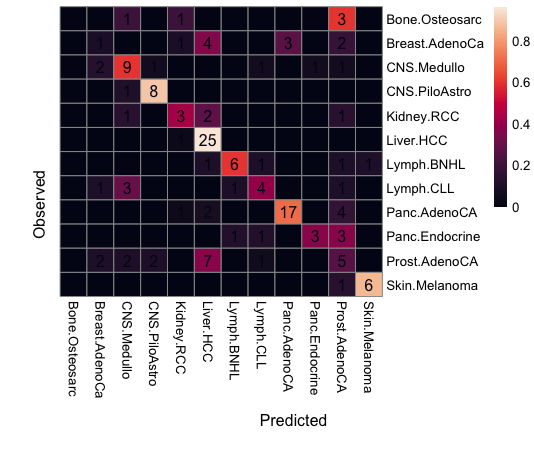
\includegraphics[width=\textwidth,height=0.9\textwidth]{graphics/confusion_matrix_bins_wasserstein.png}
    \caption{Bin/Wasserstein}
    \label{fig:confusion_bin_Wasserstein}
    \end{subfigure}
    ~
    \begin{subfigure}{.5\textwidth}
    \centering
    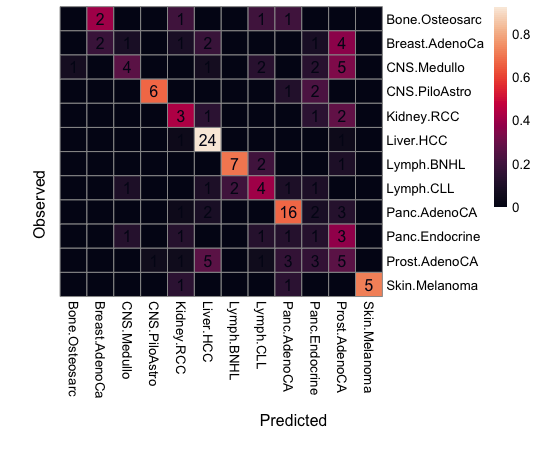
\includegraphics[width=\textwidth,height=0.9\textwidth]{graphics/confusion_matrix_smooth_wasserstein.png}
    \caption{Smooth/Wasserstein}
    \label{fig:confusion_smooth_wasserstein}
    \end{subfigure} \\
    
    \caption{\textbf{Representative confusion matrix, coloured by the percentage of predicted values over row total, for (a) Bin/Wasserstein, (b) Smooth/Wasserstein.} This is an extension of Figure \ref{ml:gle}.}
    \label{fig:apdx_ml_gle}
\end{figure}